\section{Synaptic Transmission}
There are several sources of short term synaptic plasticity

\begin{figure}[h]
\begin{center}
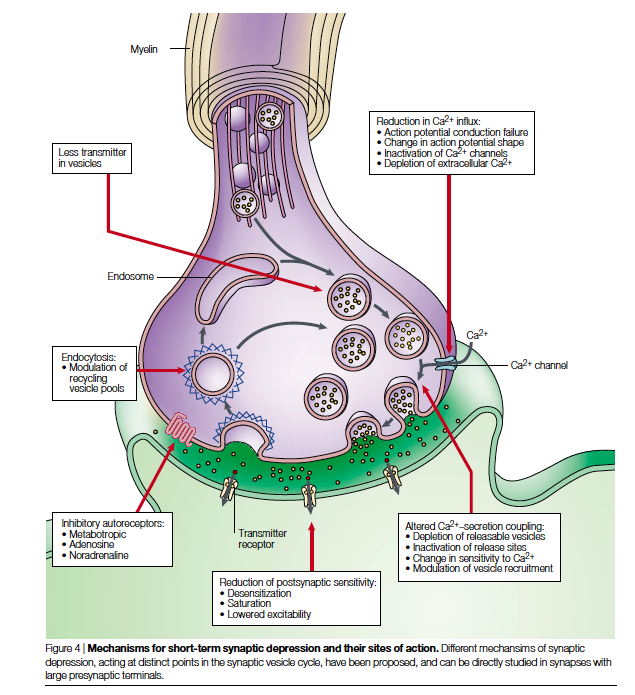
\includegraphics[scale = 0.5]{transmitionExample.png}
\end{center}
\caption{Propongo hacer una imagen similar, resaltando las principales fuentes de plasticidad o al menos las que nuestro modelo puede recuperar}
\end{figure}



\subsection{Current proportion between pre- and postsynaptic events due to difussion loss}

\begin{equation}
    	    I_s = \sum_{i=1}^{N} A_ip_i(t,rx)\Phi_i(v) = N P(t,x,r) \psi(v)
    	\end{equation}


\newpage

\section{Postsynaptic desensitization}

\subsection{Desensitization by inactivation of channels}
Under  assumption that postsynaptic channels has  activation and inactivation mechanisms, we propose    
\begin{equation}
    J_s = N p(v_{pre})d(v_{pos})\psi(v_{pos}) 
\end{equation}
where 
\begin{equation}
\partial_tp = \alpha(v_{pre})(1-p)-\beta p    
\end{equation}

While $d(v_{pos})$ and $\psi(v_{pos})$ being an inactivation  and transmembranal flux functions respectively depending on postsynaptic voltage.

\subsection{Desensitization by diminution of activation}

If we suppose that desensitization is due to a fall in activation of channels, we could model this assuming that $\alpha(v_{pre})$ is a decrease function depending on time, or any variable associated to the presynaptic mechanisms. Then the equation for synaptic current changes to: 

\begin{equation}
    J_s = N p(v_{pre})\psi(v_{pos}) 
\end{equation}
where 
\begin{equation}
\partial_tp = \alpha(v_{pre})(1-p)-\beta p    
\end{equation}
which can be rewritten as

\begin{equation}
    \partial_tp = \frac{p_{\infty}-p}{\tau_p}
\end{equation}
where 
\begin{equation}
    p_{\infty} = \frac{\alpha(v_{pre})}{\alpha(v_{pre})+\beta} 
\end{equation}

and 

\begin{equation}
    \tau_p = \frac{1}{\alpha(v_{pre}) + \beta}
\end{equation}

Function $\alpha(v_{pre})$ also can be his own dynamics and desensitization can be understood as the reach of an stable state $\alpha_{\infty}$ which is opposed to the stable estate of activation variable $p_{\infty}$. This is:
\begin{equation}
    \partial_t \alpha = \frac{\alpha_{\infty} - \alpha}{\tau_{\alpha}}
\end{equation}
where $\alpha_{\infty} = 1 - p_{\infty} $.
